\documentclass[a4paper, 12pt]{article}
\usepackage[utf8]{inputenc}
\usepackage{palatino}
\usepackage[breaklinks=true]{hyperref}
\usepackage{graphicx}
\usepackage{cprotect}
\usepackage{caption}
\usepackage[left=3cm, right=2cm, top=3cm, bottom=2cm]{geometry}
\geometry{a4paper}
\usepackage{fancyhdr}
\usepackage[brazilian]{babel}
\usepackage{siunitx}
\usepackage{subcaption}
\sisetup{detect-all}
\usepackage{float}
\usepackage{ragged2e}
\pagestyle{fancy}
\renewcommand{\headrulewidth}{0pt} 
\lhead{}\chead{}\rhead{}
\lfoot{}\cfoot{\thepage}\rfoot{}
\graphicspath{{figuras/}}
\usepackage{amsfonts}
\usepackage{mathtools}
\usepackage{cleveref}
\usepackage{spverbatim}
\usepackage[framed,numbered,autolinebreaks,useliterate]{mcode}
\setlength{\parskip}{1em}
\usepackage{xspace}
\usepackage{amsmath}
\usepackage{gensymb}
\usepackage{booktabs}
\usepackage{minted}
\usepackage{listings}
\usepackage{bm}
\usepackage{indentfirst}
\usepackage{algorithm}
\usepackage{algpseudocode, lipsum}
\lstset{
    literate={~} {$\sim$}{1}
}
\usepackage[shortlabels]{enumitem}

\newcommand{\MATLAB}{\textsc{Matlab}\xspace}
\newcommand{\SIMULINK}{\textsc{Simulink}\xspace}
\newcommand{\pspice}{\textsc{PSpice}\xspace}
\newcommand{\Python}{\textsc{Python}\xspace}
\newcommand{\tinkercad}{\textsc{TinkerCad}\xspace}
\newcommand{\arduino}{\textsc{Arduino}\xspace}
\newcommand{\sen}{\hspace{2pt}\mathrm{sen}}
\newcommand{\counts}{\textit{counts}\xspace}
\newcommand{\FT}{\text{F.T.}}
\newcommand{\zeros}{\text{Zeros}}
\newcommand{\polos}{\text{Polos}}
\newcommand{\software}{\textit{software}\xspace}
\newcommand{\hardware}{\textit{hardware}\xspace}
\newcommand{\fitness}{\textit{fitness}\xspace}
\newcommand{\fitsha}{\textit{fitness sharing}\xspace}
\newcommand{\Or}{\textbf{ou}\xspace}
\renewcommand{\Return}{\textbf{retorna}\xspace}
\newcommand{\sh}{\text{sh}\xspace}
\newcommand{\crossover}{\textit{crossover}\xspace}


\newenvironment{brprocess}[1][]
  {\begin{algorithm}[#1]
     \selectlanguage{brazilian}%
     \floatname{algorithm}{Processo}%
     \renewcommand{\algorithmicif}{\textbf{se}}%
     \renewcommand{\algorithmicfor}{\textbf{para}}%
     \renewcommand{\algorithmicdo}{\textbf{faça}}%
     \renewcommand{\algorithmicthen}{\textbf{faça}}%
     \renewcommand{\algorithmicend}{\textbf{fim}}%
     \renewcommand{\algorithmicwhile}{\textbf{enquanto}}%
     \renewcommand{\algorithmicelse}{\textbf{caso contrário}}%
     % Set other language requirements
  }
  {\end{algorithm}}

  \newenvironment{bralgorithm}[1][]
  {\begin{algorithm}[#1]
     \selectlanguage{brazilian}%
     \floatname{algorithm}{Algoritmo}%
     \renewcommand{\algorithmicif}{\textbf{se}}%
     \renewcommand{\algorithmicfor}{\textbf{para}}%
     \renewcommand{\algorithmicdo}{\textbf{faça}}%
     \renewcommand{\algorithmicthen}{\textbf{faça}}%
     \renewcommand{\algorithmicend}{\textbf{fim}}%
     \renewcommand{\algorithmicwhile}{\textbf{enquanto}}%
     \renewcommand{\algorithmicelse}{\textbf{caso contrário}}%
     % Set other language requirements
  }
  {\end{algorithm}}

\begin{document}
\begin{titlepage}
\newcommand{\HRule}{\rule{\linewidth}{0.5mm}}
	
\centering

\includegraphics[width=0.15\textwidth]{logo-unicamp.pdf}\\[0.5cm]	
\textsc{\Large Universidade Estadual de Campinas}\\[2.0cm]
\textsc{\large Faculdade de Engenharia Elétrica e de Computação}\\[0.5cm]
	
\textsc{IA707/EG507 - Computação Evolutiva}\\[2.5cm]
	
{\LARGE \bfseries EFC II}\\[3.5cm]

\begin{minipage}[t]{0.4\textwidth}
	\begin{flushleft}
    \textit{Alunos}\\
    João Pedro O. Pagnan - 199727
	\end{flushleft}
\end{minipage}
~
\begin{minipage}[t]{0.4\textwidth}
	\begin{flushright}
		\textit{Professor}\\
		Levy Boccato
	\end{flushright}
\end{minipage}\\[4.5cm]

{Campinas, \today}
	
\vfill\vfill\vfill\vfill\vfill

\includegraphics[width=0.2\textwidth]{logo-feec.png}\\[0.5cm]
\vfill 
	
\end{titlepage}

\justify

Neste exercício, vamos abordar o problema de otimização de função multimodal, com o auxílio de um algoritmo genético (GA, do inglês \textit{genetic algorithm}). Iremos considerar a função contínua
$$f (x, y) = x \cdot \sen(4\pi \cdot x) - y \cdot \sen(4\pi \cdot y + \pi) + 1,$$
onde $x, y \in [-1, 2]$ e desejamos determinar o ponto $(x^{*} , y^{*})$ que maximize a função $f(\cdot )$.
\begin{figure}[H]
    \centering
    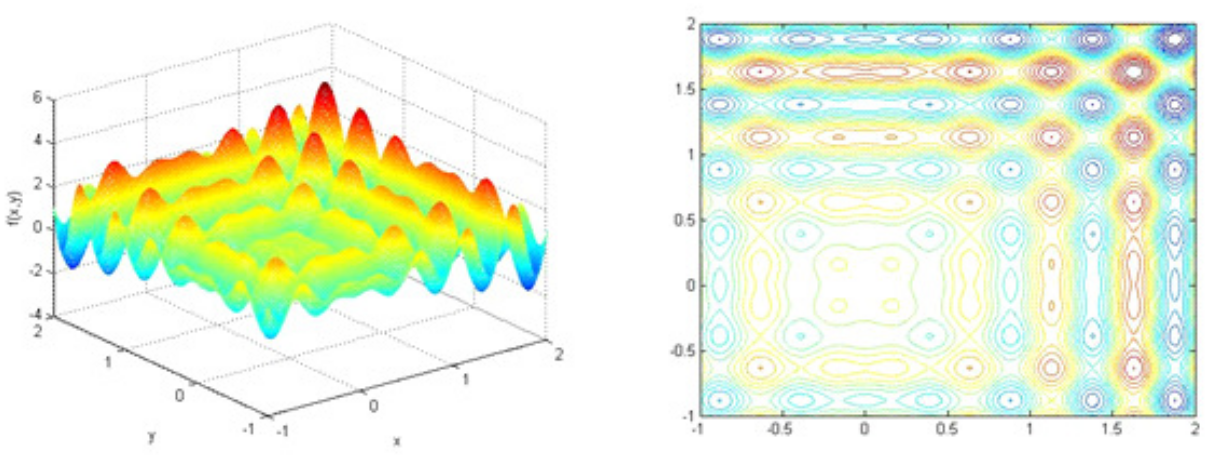
\includegraphics[width=0.8\textwidth]{figuras/grafico-funcao.png}
    \caption{Visualização da superfície e das curvas de nível da função $f (x, y)$.}
    \label{fig:grafico-funcao}
\end{figure}

\textbf{(a) Proponha um algoritmo genético (AG) para encontrar o máximo global de $f(x, y)$. Descreva todos os elementos que o compõem – codificação, função de \fitness, operadores, etc. — e justifique suas escolhas.}

O algoritmo genético para encontrar o máximo global de $f(x, y)$ será composto pelo seguinte passo a passo:
\begin{enumerate}
    \item Gerar a população inicial com $N$ indivíduos representados pela codificação adotada;
    \item Calcular o \fitness para cada indivíduo da população inicial;
    \item Aplicar o operador de seleção para selecionar dois indivíduos baseado em seus \textit{fitness};
    \item Aplicar o operador de recombinação para gerar dois descendentes;
    \item Aplicar o operador de mutação nos descendentes para que os respectivos cromossomos tenham uma probabilidade $p_m$ de serem mutados;
    \item Caso o número total de indivíduos e descendentes for menor que $2N$, repetir do passo 3 ao 5;
    \item Calcular o \fitness dos descendentes;
    \item Eliminar os $N$ indivíduos de menor \fitness;
    \item Repetir do passo 3 ao 8 até o critério de parada ser atingido.
\end{enumerate}

No caso, a codificação adotada escolhida foi a \textbf{codificação real}, em que cada indivíduo, ou solução, é representada por um vetor bidimensional cujos elementos são números reais, isto é, sendo $\bm{z}$ um indivíduo da população:
\begin{equation}
    \bm{z} = \left[x, y \right],
\end{equation}
com $x,y \in [-1, 2]$.

A \textbf{geração da população inicial} será da forma indicada no processo \ref{alg:pop-inicial}, sendo $N$ o tamanho da população.
\begin{brprocess}[!ht]
    \textbf{Paramêtros}: Tamanho da população desejada\\
    \textbf{Saída}: População gerada
    \cprotect\caption{Geração aleatória da população inicial (\verb|gerar_pop(N)|)}
    \begin{algorithmic}
    \State população $\gets [\;]$
    \State $i\gets 0$
    \While{$i < N$}
        \State cromossomo $\gets [\;]$
        \State $j \gets 0$
        \While{$j < 2$}
            \State gene $\gets$ alelo $\in [-1, 2]]$
            \State cromossomo $[j] \gets$ gene
            \State $j \gets j + 1$
        \EndWhile
        \State \textit{fitness} $\gets 0$
        \State população $[i] \gets$ [cromossomo, \textit{fitness}]
        \State $i \gets i + 1$
    \EndWhile
    \State \Return população
    \end{algorithmic}
    \label{alg:pop-inicial}
\end{brprocess}

No caso, o primeiro alelo do cromossomo se refere à variável $x$ e o segundo à variável $y$. Vale mencionar que os valores sorteados seguem uma distribuição uniforme.

\textbf{Observação:} Como o algoritmo genético será implementado em \Python, foi considerado que a coordenadas dos elementos dos vetores se iniciam em 0.

Na segunda etapa do algoritmo genético tem-se o \textbf{cálculo do valor da função de avaliação}. No caso, a função de avaliação, ou \fitness, adotada é a própria função que deseja-se maximizar. Dessa forma, o cálculo é dado por:
\begin{equation}\label{eq:fitness}
    \phi(\bm{z}) = \phi(x, y) = x \cdot \sen(4\pi \cdot x) - y \cdot \sen(4\pi \cdot y + \pi) + 1
\end{equation}

Com isso, o processo que define o cálculo do \fitness é descrito da forma indicada no processo \ref{alg:fitness}.
\begin{brprocess}[!ht]
\textbf{Entradas}: população\\
\textbf{Saída}: população com os valores de \fitness atualizado
\cprotect\caption{Cálculo do \fitness (\verb|calc_fitness(populacao)|)}
\begin{algorithmic}
\For{indivíduo \textbf{em} população}
    \If{indivíduo[1] = 0}
        \State{$x =$ indivíduo$[0][0]$}
        \State{$y =$ indivíduo$[0][1]$}
        \State{\fitness = $x \cdot \sen(4\pi \cdot x) - y \cdot \sen(4\pi \cdot y + \pi) + 1$}
        \State indivíduo[1] = \fitness
    \EndIf
\EndFor
\State \Return população
\end{algorithmic}
\label{alg:fitness}
\end{brprocess}

Na terceira etapa, o GA aplica o \textbf{operador de seleção por torneio} na população. Esse método utiliza o parâmetro $q$, que é igual à quantidade de indivíduos da população selecionados por torneio. Esse método é executado duas vezes no algoritmo genético, de forma a determinar dois pais para a recombinação e é descrito pelo processo \ref{alg:selecao}.
\begin{brprocess}[!ht]
    \cprotect\caption{Operador de seleção por torneio (\verb|selecao_torneio(populacao,|
    \verb|N, q_torneio)|}
    \textbf{Entrada:} população\\
    \textbf{Parâmetros}: quantidade de indivíduos da população selecionados por torneio e tamanho da população inicial\\
    \textbf{Saída}: o melhor indivíduo escolhido no torneio
    \begin{algorithmic}
            \State $i \gets 0$
            \State indivíduos participantes $\gets [\;]$
            \While{$i < q$}
                \State índice indivíduo selecionado $\gets n \in \{0, 1, ..., N - 1\}$
                \State indivíduos participantes $[i] \gets$ população [índice indivíduo selecionado]
                \State $i \gets i + 1$
            \EndWhile
            \State índice do melhor indivíduo $\gets$ indivíduos participantes[\verb|argmax|(indivíduos participantes [:,1]])
            \State melhor indivíduo $\gets$ indivíduos participantes[índice do melhor indivíduo]
            \State \Return melhor indivíduo
    \end{algorithmic}
    \label{alg:selecao}
\end{brprocess}

Este operador foi escolhido por possibilitar o ajuste da pressão seletiva na população através do parâmetro $q$.

Em seguida, na quarta etapa, o \textbf{operador de recombinação} escolhido foi o método de \textit{crossover} aritmético. Nele, os filhos gerados resultam de uma combinação linear dois pais. Esse método foi escolhido por ser bem apropriado para problemas de otimização numérica com restrições onde a região factível é convexa. Esse é o caso para o problema que deseja-se resolver.

O operador de recombinação escolhido é descrito pelo processo \ref{alg:recombinacao}. Vale ressaltar que o valor aleatório $a$ é obtido através de uma realização de um processo com distribuição uniforme e $a \in [0, 1]$. 
\begin{brprocess}[!ht]
    \cprotect\caption{Operador de recombinação (\verb|crossover_aritmetico(cromossomo_p1,|
    \verb|cromossomo_p2|)}
    \textbf{Entrada}: cromossomo dos dois pais\\
    \textbf{Saída}: cromossomo de ambos os filhos
    \begin{algorithmic}
        \State $i \gets 0$
        \State descendentes $\gets [\;]$
        \State $a \gets \text{número aleatório} \in [0, 1]$
        \While{$i < 2$}
            \If{$i = 0$}
                \State filho $\gets a \cdot \text{pai}_1 + (1 - a) \cdot \text{pai}_2$
            \EndIf
            \If{$i = 1$}
                \State filho $\gets (1 - a) \cdot \text{pai}_1 + a \cdot \text{pai}_2$
            \EndIf
            \State descendentes[$i$] $\gets$ filho
            \State $i \gets i + 1$
        \EndWhile
        \State \Return descendentes
    \end{algorithmic}
    \label{alg:recombinacao}
\end{brprocess}

Por fim, resta detalhar o \textbf{operador de mutação} utilizado. Considerando um indivíduo $x \in \mathbb{R}^2$, seu valor mutado pode ser expresso por $x' = m(x)$, sendo $m(\cdot)$ o operador de mutação. 

No caso, foi escolhida a \textbf{mutação uniforme}. Logo, pode-se descrever a mutação através da expressão $x' = x + M$, com $M$ sendo um vetor de variáveis aleatórias no $\mathbb{R}^2$ e seguindo uma distribuição aleatória uniforme $U = (a, b)^2$. As variáveis $a$ e $b$ são os limites inferiores e superiores da região de busca, respectivamente, de forma que $a = -1$ e $b = 2$.

O processo pode ser descrito da forma indicada no processo \ref{alg:mutacao}, sendo $p_m$ a probabilidade da mutação ocorrer.
\begin{brprocess}[!ht]
    \cprotect\caption{Operador de mutação (\verb|mutacao_uniforme(cromossomo|,
    \verb|p_mutacao|, \verb|a|, \verb|b|)}
    \textbf{Entrada}: cromossomo a ser mutado e valores máximos e mínimos do espaço de busca\\
    \textbf{Parâmetros}: probabilidade da mutação ocorrer\\
    \textbf{Saída}: cromossomo mutado
    \begin{algorithmic}
        \State{k $\gets$ número aleatório $\in [0, 1]$}
        \If{$k < p_m$}
            \State{$M \gets []$}
            \State{$i \gets 0$}
            \While{$i < 2$}
                \State{$M[i] \gets$ número aleatório $\in [a, b]$}
                \State{cromossomo$[i] \gets$ cromossomo$[i] + M[i]$}
                \If{cromossomo$[i] < a$}
                    \State{cromossomo$[i] \gets a$}
                \EndIf
                \If{cromossomo$[i] > b$}
                    \State{cromossomo$[i] \gets b$}
                \EndIf
                \State{$i \gets i + 1$}
            \EndWhile
        \EndIf
        \State \Return cromossomo
    \end{algorithmic}
    \label{alg:mutacao}
\end{brprocess}

Com isso, foram descritos os operadores escolhidos para serem utilizados na geração, seleção, recombinação e mutação de indivíduos desse algoritmo genético.

Esses operadores serão executados nessa sequência até que a população tenha $2N$ soluções, quando ocorrerá uma eliminação dos $N$ indivíduos de menor \textit{fitness}, sendo que o processo será repetido até o critério de parada ser atingido. 

O \textbf{critério de parada} escolhido para o algoritmo foi o número de gerações $n_g$. 

Esse algoritmo tem, portanto, os seguintes parâmetros:
\begin{itemize}
    \item $N$: tamanho da população inicial;
    \item $q$: quantidade de indivíduos presentes no torneio;
    \item $p_m$: probabilidade de ocorrer uma mutação;
    \item $n_g$: número de gerações.
    \item $a$: menor valor do espaço de busca;
    \item $b$: maior valor do espaço de busca;
\end{itemize}

O valor de cada parâmetro foi determinado de maneira exploratória, sendo que os valores escolhidos estão indicados na tabela \ref{tab:valores-parametros}. Vale ressaltar que os valores mínimo e máximo do espaço de busca já estão estabelecidos no enunciado do problema que deseja-se resolver.
\begin{table}[H]
    \centering
    \begin{tabular}{c c}
    \toprule
        $\bm{N}$ & 500\\
        $\bm{q}$ & 5\\
        $\bm{p_m}$ & 0.2\\
        $\bm{n_g}$ & 20\\
        $\bm{a}$ & -1\\
        $\bm{b}$ & 2\\
    \bottomrule
    \end{tabular}
    \caption{Valores para os parâmetros do algoritmo genético.}
    \label{tab:valores-parametros}
\end{table}

Desta forma, tem-se o algoritmo genético desenvolvido para a encontrar o ponto de máximo da expressão $f(x, y)$ na região solicitada.

\textbf{(b) Para cada uma de 5 execuções independentes do AG, apresente as curvas de \fitness médio e de \fitness do melhor indivíduo em função do número de gerações. Mostre também, tendo por pano de fundo as curvas de nível da função $f(x, y)$, a distribuição dos indivíduos da população final em cada execução. Com base nesse conjunto de gráficos, busque analisar o algoritmo em termos de sua eficiência de busca e manutenção de diversidade.}

Executando o algoritmo genético desenvolvido cinco vezes, obtiveram-se as curvas de melhor \fitness, \fitness médio e, ao lado dessas figuras, estão apresentadas as distribuições das populações finais sobre as curvas de nível de $f(x,y)$ em cada realização, como indicado na figura \ref{fig:fitness-distribuicao}.
\begin{figure}[!ht]
    \centering
    \begin{subfigure}{0.4\textwidth}
        \includegraphics[width=\textwidth]{figuras/algoritmo-genetico/fitness-realizacao-1.pdf}
    \end{subfigure}
    \begin{subfigure}{0.4\textwidth}
        \includegraphics[width=\textwidth]{figuras/algoritmo-genetico/distribuicao-realizacao-1.pdf}
    \end{subfigure}
    \hfill
    \\
    \centering
    \begin{subfigure}{0.4\textwidth}
        \includegraphics[width=\textwidth]{figuras/algoritmo-genetico/fitness-realizacao-2.pdf}
    \end{subfigure}
    \begin{subfigure}{0.4\textwidth}
        \includegraphics[width=\textwidth]{figuras/algoritmo-genetico/distribuicao-realizacao-2.pdf}
    \end{subfigure}
    \hfill
    \\
    \centering
    \begin{subfigure}{0.4\textwidth}
        \includegraphics[width=\textwidth]{figuras/algoritmo-genetico/fitness-realizacao-3.pdf}
    \end{subfigure}
    \begin{subfigure}{0.4\textwidth}
        \includegraphics[width=\textwidth]{figuras/algoritmo-genetico/distribuicao-realizacao-3.pdf}
    \end{subfigure}
    \hfill
    \\
    \centering
    \begin{subfigure}{0.4\textwidth}
        \includegraphics[width=\textwidth]{figuras/algoritmo-genetico/fitness-realizacao-4.pdf}
    \end{subfigure}
    \begin{subfigure}{0.4\textwidth}
        \includegraphics[width=\textwidth]{figuras/algoritmo-genetico/distribuicao-realizacao-4.pdf}
    \end{subfigure}
    \hfill
    \\
    \centering
    \begin{subfigure}{0.4\textwidth}
        \includegraphics[width=\textwidth]{figuras/algoritmo-genetico/fitness-realizacao-5.pdf}
    \end{subfigure}
    \begin{subfigure}{0.4\textwidth}
        \includegraphics[width=\textwidth]{figuras/algoritmo-genetico/distribuicao-realizacao-5.pdf}
    \end{subfigure}
    \hfill
    \caption{À esquerda, as curvas de melhor \fitness e \fitness médio em cada realização e, à direita, a distribuição da população final sobre as curvas de nível de $f(x, y)$ nas respectivas realizações.}
    \label{fig:fitness-distribuicao}
\end{figure}

É possível notar que, na maior parte das realizações do algoritmo a curva de \fitness médio se aproxima à de melhor \fitness com o aumento do número da geração que este está. No caso, o valor médio e desvio padrão obtidos para a função de avaliação utilizando as melhores soluções de cada realização foi de $\num{4.2475709055\pm 0.0126350757}$ e, combinando este resultado a uma análise do gráfico, nota-se que o algoritmo foi bem sucedido em encontrar o máximo de $f(x,y)$ no intervalo solicitado.

Apesar disso, nota-se que há pouca diversidade na população final, afinal, a distri\-buição dos indivíduos sobre as curvas de nível de $f(x,y)$ não é tão grande, indicando que as soluções estão se assemelhando bastante umas com as outras.

Neste caso, isso não foi um problema porque todas as melhores soluções foram para a mesma região da superfície, mas, caso a função que deseja-se maximizar fosse diferente, as melhores soluções poderiam ir para máximos locais da região analisada.

Desta forma, conclui-se que, apesar do algoritmo ser eficiente em termos de sua eficiência de busca, esse não é eficiente para manter a diversidade da população. 

\textbf{(c) Implemente agora o método de \fitsha. Comente as escolhas feitas para os valores dos parâmetros (e.g., $\sigma_s$) e de operadores (caso alguma modificação em relação ao item (b) tenha sido necessária). Repita o procedimento do item (b) para analisar o comportamento do \fitsha.}

O \fitsha consiste na técnica de indivíduos "similares" compartilhar o \fitness, de forma que a quantidade de indivíduos em uma localidade ser limitada pelo valor da função de avaliação daquela região.

De forma resumida, o compartilhamento acontece por meio da redução do \fitness puro dos indivíduos por um fator proporcional à quantidade de indivíduos similares na população, ou seja, o \fitness compartilhado de um indivíduo $x_i$ resulta da divisão do valor puro da função de avaliação $f(x_i)$ por um contador de nichos $c_i$, que mede o número de indivíduos com os quais $i$ compartilha o valor de \fitness, como dado na equação  \ref{eq:fitsha}.
\begin{equation}\label{eq:fitsha}
    \overline{f} (x_i) = \frac{f(x_i)}{c_i}
\end{equation}

O contador de nichos $c_i$ é dado por \ref{eq:fitshaci}, sendo $\sh(\cdot)$ a função de compartilhamento.
\begin{equation}\label{eq:fitshaci}
    c_i = \sum_{j=1}^N \sh (d(x_i, x_j))
\end{equation}

Utilizando a expressão dada em \cite{goldberg1987genetic} para a função de compartilhamento, construiu-se o algoritmo apresentado no processo \ref{proc:fitsha} para o \fitsha. No caso, a medida de distância utilizada é a distância euclidiana entre os indivíduos $i$ e $j$ no plano $xy$.  
\begin{brprocess}[!ht]
    \cprotect\caption{Operador de \fitsha (\verb|fitness_sharing(população,|
    \verb|sigma, alpha|)}
    \textbf{Entrada}: população para atualizar o \fitsha\\
    \textbf{Parâmetros}: $\sigma_s$ e $\alpha_s$ \\
    \textbf{Saída}: população com a métrica de \fitsha calculada
    \begin{algorithmic}
    \For{indivíduo \textbf{em} população}
        \If{indivíduo[2] = 0}
            \State similaridade $\gets [\;]$
            \State $i \gets 0$
            \While{$i <$ \verb|len(populacao|)}            
                \State{distância $\gets$ \verb|calc_distância(indivíduo[0], população[i][0]|}
                \If{distância $< \sigma_s$}
                    \State {similaridade$[i]$ $\gets 1 - (\frac{\text{distância}}{\sigma_s})^{\alpha_s}$}                
                \Else
                    \State {similaridade$[i]$ $\gets$ 0}
                \EndIf       
                \State $i \gets i + 1$
            \EndWhile      
            \State \fitsha $\gets \frac{\text{individuo}[1]}{\sum(\text{similaridade})}$
            \State {indivíduo[2] $\gets$ \fitsha}
        \EndIf
        \EndFor
        \State \textbf{retorna} população
    \end{algorithmic}
    \label{proc:fitsha}
\end{brprocess}

Vale mencionar também que, agora, a seleção por torneio é realizada utilizando o \fitsha, assim como a seleção dos indivíduos que irão sobreviver.  

Esse novo método tem os seguintes novos parâmetros:
\begin{itemize}
    \item $\sigma_s$: limiar de similaridade;
    \item $\alpha_s$: regulação da forma da função.
\end{itemize}

O valor de cada parâmetro foi determinado de maneira exploratória, sendo que os valores escolhidos estão indicados na tabela \ref{tab:valores-parametros2}. Vale ressaltar que, os valores dos outros parâmetros continuam iguais, de forma a realizar uma comparação entre quando o método de \fitsha é utilizado ou não.
\begin{table}[H]
    \centering
    \begin{tabular}{c c}
    \toprule
        $\bm{\sigma}_s$ & 0.4\\
        $\bm{\alpha}_s$ & 1\\
    \bottomrule
    \end{tabular}
    \caption{Valores dos novos parâmetros introduzidos.}
    \label{tab:valores-parametros2}
\end{table}

Implementando o \fitsha utilizando o processo \ref{proc:fitsha} e executando o algoritmo genético cinco vezes, obtiveram-se os resultados apresentados na figura \ref{fig:fitness-distribuicao-sharing}.
\begin{figure}[!ht]
    \centering
    \begin{subfigure}{0.4\textwidth}
        \includegraphics[width=\textwidth]{figuras/fitness-sharing/fitness-realizacao-1.pdf}
    \end{subfigure}
    \begin{subfigure}{0.4\textwidth}
        \includegraphics[width=\textwidth]{figuras/fitness-sharing/distribuicao-realizacao-1.pdf}
    \end{subfigure}
    \hfill
    \\
    \centering
    \begin{subfigure}{0.4\textwidth}
        \includegraphics[width=\textwidth]{figuras/fitness-sharing/fitness-realizacao-2.pdf}
    \end{subfigure}
    \begin{subfigure}{0.4\textwidth}
        \includegraphics[width=\textwidth]{figuras/fitness-sharing/distribuicao-realizacao-2.pdf}
    \end{subfigure}
    \hfill
    \\
    \centering
    \begin{subfigure}{0.4\textwidth}
        \includegraphics[width=\textwidth]{figuras/fitness-sharing/fitness-realizacao-3.pdf}
    \end{subfigure}
    \begin{subfigure}{0.4\textwidth}
        \includegraphics[width=\textwidth]{figuras/fitness-sharing/distribuicao-realizacao-3.pdf}
    \end{subfigure}
    \hfill
    \\
    \centering
    \begin{subfigure}{0.4\textwidth}
        \includegraphics[width=\textwidth]{figuras/fitness-sharing/fitness-realizacao-4.pdf}
    \end{subfigure}
    \begin{subfigure}{0.4\textwidth}
        \includegraphics[width=\textwidth]{figuras/fitness-sharing/distribuicao-realizacao-4.pdf}
    \end{subfigure}
    \hfill
    \\
    \centering
    \begin{subfigure}{0.4\textwidth}
        \includegraphics[width=\textwidth]{figuras/fitness-sharing/fitness-realizacao-5.pdf}
    \end{subfigure}
    \begin{subfigure}{0.4\textwidth}
        \includegraphics[width=\textwidth]{figuras/fitness-sharing/distribuicao-realizacao-5.pdf}
    \end{subfigure}
    \hfill
    \caption{À esquerda, as curvas de melhor \fitness e \fitness médio em cada realização e, à direita, a distribuição da população final sobre as curvas de nível de $f(x, y)$ nas respectivas realizações.}
    \label{fig:fitness-distribuicao-sharing}
\end{figure}

Com o \fitsha, nota-se uma grande mudança na distribuição da população final sobre as curvas de nível de $f(x, y)$, assim como nas curvas de \fitness médio nas realizações, sendo que apenas as curvas de melhor \fitness se mantiveram como antes, indicando que a solução ótima ainda está na população final. Além disso, nas figuras das distribuições, nota-se que as populações finais estão distribuídas ao redor dos máximos locais da superfície, evidenciando o diferente resultado obtido com a implementação do \fitsha.

Quando observa-se o valor médio e o desvio padrão nas realizações para quando a seleção foi feita com o \fitsha, essa mudança é realçada. No caso, o \fitness médio e o desvio padrão obtido com as cinco realizações quando utiliza-se como critério o \fitsha cai para $1.3957084514\pm 0.4094684937$.

À princípio, analisando de uma forma puramente métrica, o \fitsha dá a impressão de fornecer maus resultados para a população final do algoritmo genético, mas, analisando de um ponto de vista da engenharia, o \fitsha aumenta, em muito, a diversidade da população final. 

Isso é de extrema importância quando a solução ótima tem um custo muito elevado para ser implementada. Agora, quando se tem vários ótimos locais no conjunto final de soluções, encontrar uma que possa ser implementada sem trazer tantos custos para o projeto de engenharia fica consideravelmente mais fácil. Esse não era o caso para o problema em análise, mas é algo que deve ser levado em conta para resolver certos tipos de problemas de engenharia com computação evolutiva. 

Com isso, vê-se a importância de técnicas de \fitsha na resolução de problemas.

\textbf{(d) Introduza, por fim, o esquema de restrição de cruzamento (seguindo o espírito da abordagem de especiação) proposto por \cite{deb1989genetic} Analise o impacto da inserção deste mecanismo na evolução da população e, em última análise, no desempenho do algoritmo.}

Adicionando o esquema de restrição de cruzamento pela abordagem de especiação no algoritmo genético com \fitsha. 

Esse método funciona restringindo a recombinação entre indivíduos utilizando a distância entre eles, de forma que apenas indivíduos limitados a uma distância de $\sigma_{mate}$ poderão gerar descendentes. No caso, se a distância for maior que $\sigma_{mate}$, um novo sorteio é realizado e, caso toda a população seja varrida para procurar outro par com base na distância, um indivíduo aleatório é sorteado, desconsiderando essa métrica.

Logo, a única alteração que haverá no algoritmo será na recombinação, que agora só será realizada se a distância entre os indivíduos é menor que $\sigma_{mate}$ e, caso contrário, uma nova seleção é feita até encontrar indivíduos compatíveis, considerando também o \fitsha, como mostrado no processo \ref{alg:especiacao}.
\begin{brprocess}[!ht]
    \cprotect\caption{Operador de especiação (\verb|especiacao(individuo_1,|
    \verb|individuo_2, sigma_mate|)}
    \textbf{Entrada}: cromossomo dos dois pais\\
    \textbf{Parâmetros}: $\sigma_{mate}$ \\
    \textbf{Saída}: cromossomo de ambos os filhos
    \begin{algorithmic}
        \State distância $\gets$ \verb|calc_distância(individuo_1, individuo_2)|
        \If{distância $< \sigma_{mate}$}
            \State \Return 1
        \Else
            \State \Return 0
        \EndIf
    \end{algorithmic}
    \label{alg:especiacao}
\end{brprocess}

Para este operador, foi 

Executando o algoritmo genético com \fitsha e especiação, obtiveram-se os resultados apresentados na figura \ref{fig:fitness-distribuicao-sharing-especiacao}.
\begin{figure}[!ht]
    \centering
    \begin{subfigure}{0.4\textwidth}
        \includegraphics[width=\textwidth]{figuras/especiacao/fitness-realizacao-1.pdf}
    \end{subfigure}
    \begin{subfigure}{0.4\textwidth}
        \includegraphics[width=\textwidth]{figuras/especiacao/distribuicao-realizacao-1.pdf}
    \end{subfigure}
    \hfill
    \\
    \centering
    \begin{subfigure}{0.4\textwidth}
        \includegraphics[width=\textwidth]{figuras/especiacao/fitness-realizacao-2.pdf}
    \end{subfigure}
    \begin{subfigure}{0.4\textwidth}
        \includegraphics[width=\textwidth]{figuras/especiacao/distribuicao-realizacao-2.pdf}
    \end{subfigure}
    \hfill
    \\
    \centering
    \begin{subfigure}{0.4\textwidth}
        \includegraphics[width=\textwidth]{figuras/especiacao/fitness-realizacao-3.pdf}
    \end{subfigure}
    \begin{subfigure}{0.4\textwidth}
        \includegraphics[width=\textwidth]{figuras/especiacao/distribuicao-realizacao-3.pdf}
    \end{subfigure}
    \hfill
    \\
    \centering
    \begin{subfigure}{0.4\textwidth}
        \includegraphics[width=\textwidth]{figuras/especiacao/fitness-realizacao-4.pdf}
    \end{subfigure}
    \begin{subfigure}{0.4\textwidth}
        \includegraphics[width=\textwidth]{figuras/especiacao/distribuicao-realizacao-4.pdf}
    \end{subfigure}
    \hfill
    \\
    \centering
    \begin{subfigure}{0.4\textwidth}
        \includegraphics[width=\textwidth]{figuras/especiacao/fitness-realizacao-5.pdf}
    \end{subfigure}
    \begin{subfigure}{0.4\textwidth}
        \includegraphics[width=\textwidth]{figuras/especiacao/distribuicao-realizacao-5.pdf}
    \end{subfigure}
    \hfill
    \caption{À esquerda, as curvas de melhor \fitness e \fitness médio em cada realização e, à direita, a distribuição da população final sobre as curvas de nível de $f(x, y)$ nas respectivas realizações.}
    \label{fig:fitness-distribuicao-sharing-especiacao}
\end{figure}


\clearpage

\bibliographystyle{ieeetr}

\bibliography{bib}

\pdfinfo{
   /Title  (IA707 - EFC II - 199727)
}
 \end{document}